\documentclass[12pt,letterpaper]{article}
\usepackage{fullpage}
\usepackage[top=2cm, bottom=4.5cm, left=2.5cm, right=2.5cm]{geometry}
\usepackage{amsmath,amsthm,amsfonts,amssymb,amscd}
\usepackage{lastpage}
\usepackage{enumerate}
\usepackage{fancyhdr}
\usepackage{mathrsfs}
\usepackage{xcolor}
\usepackage{graphicx}
\usepackage{listings}
\usepackage{mcode}
\usepackage{hyperref}
\usepackage{movie15}
\usepackage{hyperref}
\usepackage{float}


% \hypersetup{%
%   colorlinks=true,
%   linkcolor=blue,
%   linkbordercolor={0 0 1}
% }
 
% \renewcommand\lstlistingname{Algorithm}
% \renewcommand\lstlistlistingname{Algorithms}
% \def\lstlistingautorefname{Alg.}

% \lstdefinestyle{Python}{
%     language        = Python,
%     frame           = lines, 
%     basicstyle      = \footnotesize,
%     keywordstyle    = \color{blue},
%     stringstyle     = \color{green},
%     commentstyle    = \color{red}\ttfamily
% }

\setlength{\parindent}{0.0in}
\setlength{\parskip}{0.05in}

% Edit these as appropriate
\newcommand\course{Signal Processing}
\newcommand\hwnumber{1}                  % <-- homework number
\newcommand\NetIDa{Mehdi Raza}           % <-- NetID of person #1
\newcommand\NetIDb{}           % <-- NetID of person #2 (Comment this line out for problem sets)

\pagestyle{fancyplain}
\headheight 35pt
\lhead{\NetIDa}
\lhead{\NetIDa\\\NetIDb}                 % <-- Comment this line out for problem sets (make sure you are person #1)
\chead{\textbf{\Large Homework \hwnumber}}
\rhead{\course \\ \today}
\lfoot{}
\cfoot{}
\rfoot{\small\thepage}
\headsep 1.5em

\begin{document}

\section*{Question 1}
\subsection*{Part (a)}
The sketch is given as follows: 
\begin{figure}[h]
    \centering
    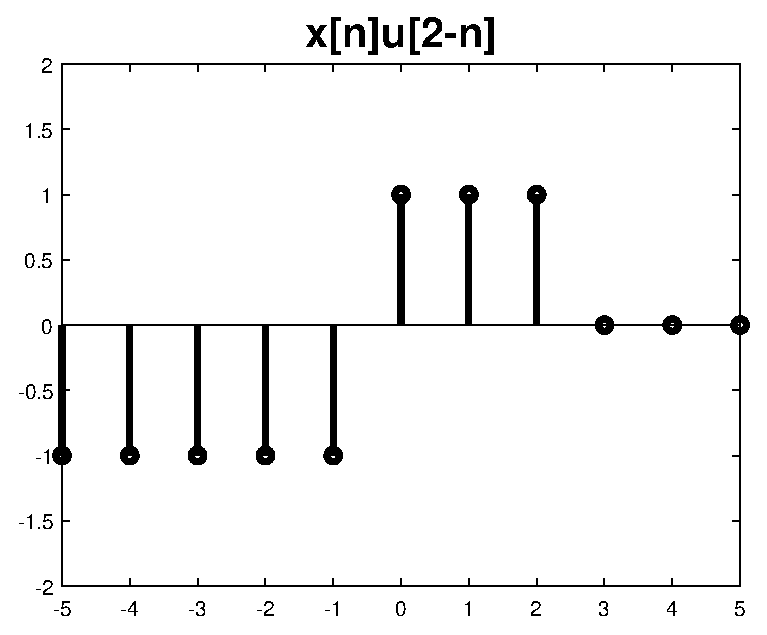
\includegraphics{figures/1a.eps}
    \caption{part (a) plot}
    \label{1a}
\end{figure}

\subsection*{Part (b)}
The sketch is given as follows: 
\begin{figure}[h]
    \centering
    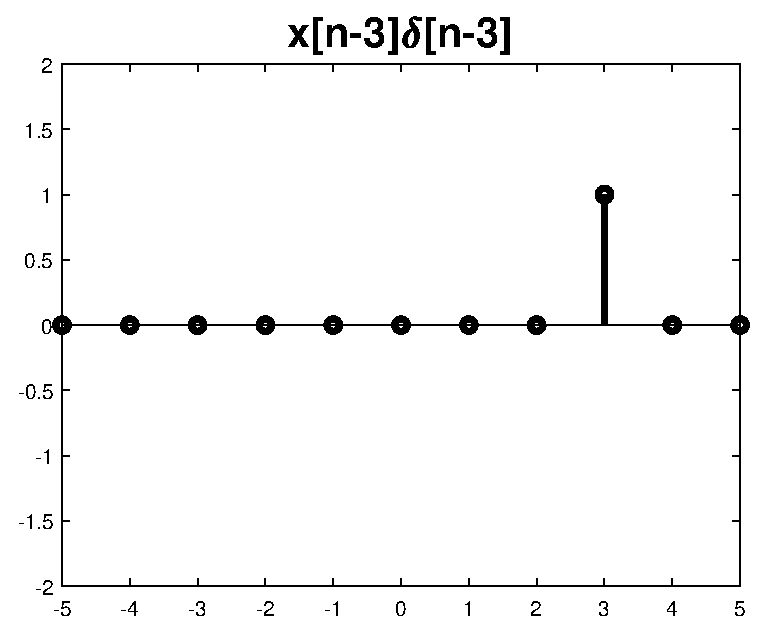
\includegraphics{figures/1b.eps}
    \caption{part (b) plot}
    \label{1b}
\end{figure}

\pagebreak 
\section*{Question 2}
\subsection*{Part (a)}
Given:
    \[
    y[n] = x[-(n-2)]
    \]
\begin{enumerate}
    \item \textbf{Memorylessness:} The system is not memoryless as $y[n]$ depends on $x[2-n]$. 
    \item \textbf{Causality:}
    We present a counter example to prove system is non-causal. For $n < 0$ we see that the system depends on future values i.e.:
    \[
    n<0 \implies n-2 < -2 \implies -(n-2) > 2
    \]
    That is to say, for all negative values of n, the system depends on $n > 2$. Hence it is non-causal. 
    \item \textbf{Linear:} Assume 2 arbitrary inputs $a x_1[n]$ and $bx_2[n]$ ($a$, $b$ are constants). Their individual responses are as:
    \[
    y_1[n] = a x_1[2-n]
    \]
    and 
    \[
    y_2[n] = b x_2[2-n]
    \]
    On the other hand, summing the inputs first and then calculating their responses:
    \[
    x[n] = a x_1[n] + b x_2[n]
    \]
    Since time shifting and scaling are distributive (the system is only performing these two operations), we have: 
    \[
        y[n] = a y_1[n] + by_2[n]
    \]
    System is linear. 
    
    \item \textbf{Time Invariant:}
    let us define an input $x_1[n-n_o]$. Applying it to the system, we get: 
    \[
        y_1[n] = x[2- (n-n_o)]
    \]
    % \[
    %     y_1[n] = x[2- n + n_o]
    % \]
    Now, we shift $y[n]$ by $n_o$:
    \[
        y[n-n_o] = x[2- (n-n_o)]
    \]
    Since both are same, the system is time invariant. 
    
    \item \textbf{Stable:} For a bounded input $-B_x<x[n]<B_x$, the system is just shifting and time reversing the input signal. Hence: 
    \[
        -B_y < y[n] = x[2-n] < B_y
    \]
    System is stable. 
    
\end{enumerate}

\subsection*{Part (b)}
Given:
    \[
    y[n] = nx[-n]
    \]
\begin{enumerate}
    \item \textbf{Memorylessness:} The system is not memoryless as $y[n]$ depends on $x[-n]$. 
    \item \textbf{Causality:}
    System is non-causal as it depends on future values for $n<0$
    \item \textbf{Linear:} Assume 2 arbitrary inputs $a x_1[n]$ and $bx_2[n]$ ($a$, $b$ are constants). Their individual responses are as:
    \[
    y_1[n] = a n x_1[-n]
    \]
    and 
    \[
    y_2[n] = b n x_2[-n]
    \]
    On the other hand, summing the inputs first and then calculating their responses:
    \[
    x[n] = a x_1[n] + b x_2[n]
    \]
    \[
        y[n] = n (a x_1[-n] + b x_2[-n])
    \]
    \[
        y[n] = a n x_1[-n] + b n x_2[-n]
    \]
    Since: 
    \[
        y[n] = y_1[n] + y_2[n]
    \]
    System is linear. 
    
    \item \textbf{Time Invariant:}
    let us define an input $x_1[n-n_o]$. Applying it to the system, we get: 
    \[
        y_1[n] = n x[-(n-n_o)]
    \]
    % \[
    %     y_1[n] = x[2- n + n_o]
    % \]
    Now, we shift $y[n]$ by $n_o$:
    \[
        y[n-n_o] = (n-n_o)x[- (n-n_o)]
    \]
    Since both are \textbf{not} same, the system is time variant. 
    
    \item \textbf{Stable:} For a bounded input $-B_x<x[n]<B_x$: 
    \[
        y[n] = n x[2-n]
    \]
    The output is not bounded, hence system is not stable. 
    
\end{enumerate}
\pagebreak

\section*{Question 3}
Reversing and shifting the impulse response $h$ by $n$ and plotting as a function of $k$ in figure \ref{conv_sum}. 
\begin{figure}[h]
    \centering
    \includegraphics{figures/3in.png}
    \caption{convolution sum}
    \label{conv_sum}
\end{figure}
\begin{figure}[h]
    \centering
    \includegraphics{figures/3.eps}
    \caption{Convolution output}
    \label{conv}
\end{figure}

The convolution is then calculated as  follows:
\begin{itemize}
    \item For $n < 0$:\\
    Since there is no overlap, 
    \[
        y[n] = 0
    \]
    \item  For $0 \leq n \leq 4$:\\
    Overlap exists, 
    \[
    \begin{bmatrix}
        y[0]\\
        y[1]\\
        y[2]\\
        y[3] \\
        y[4]\\
    \end{bmatrix}= 
    \begin{bmatrix}
     1\\
     -1 + 1 \\
     -2 + 1\\
     -2\\
     -1
    \end{bmatrix}
=
\begin{bmatrix}
     1\\
     0 \\
     -1\\
     -2\\
     -1
    \end{bmatrix}
    \]
    
    \item For $n > 4$:\\
    No overlap, 
    \[
        y[n] = 0
    \]
\end{itemize}
Figure \ref{conv} summarizes the convolution results.
% \begin{figure}[h]
%     \centering
%     \includegraphics{figures/3.eps}
%     \caption{Convolution output}
%     \label{conv}
% \end{figure}
\pagebreak
\section*{Question 4}
\subsection*{Part (a)}
Given: 
\[
    h[n] = \delta[n] - \delta[n-1] +\delta[n+1]
\]
\subsubsection*{Causality}
Inspecting the given impulse response, we see that it is non zero when $n<0$ due to presence of an impulse i.e.: 
\[
    h[n] = \dots \delta[n+1]
\]
Hence system is non-causal.
\subsubsection*{Stability}
For stability, check for absolute summability: 
\[
    \sum_{k = -\infty} ^ {k=\infty} | h[k] |< \infty
\]
Since $h[n]$ is non zero at 3 points, the summation reduces to:
\[
  \sum_{k = -\infty} ^ {k=\infty} | h[k] | =  1-1+1 = 1 < \infty
\]
Hence system is stable.


% For stability, we calculate the system's response for any arbitrary but bounded input :
% \[
%     x[n] \leq B_x
% \]
% To calculate system's response, we use convolution sum as follows: 
% \[
%     y[n] = \sum_{k = -\infty}^{k = +\infty} x[k] (\delta[n-k] - \delta[n-k-1] + \delta[n-k+1])
% \]
% Using the sampling property of $\delta[n]$, we get: 
% \[
%     y[n] = \sum_{k = -\infty}^{k = +\infty} x[k]\delta[n-k] - x[k+1]\delta[n-k-1] + x[k-1]\delta[n-k+1])
% \]
% \[
%     \because \delta[n] = 1
% \]
% \[
%     y[n] = \sum_{k = -\infty}^{k = +\infty} x[k] - x[k+1] + x[k-1]
% \]
% The above expression indicates that $y[n]$ is bounded iff $x[k]$'s magnitude decreases with time or $x[n]$ is \textbf{not} nonzero \textbf{for all} values of $n$.


\subsection*{Part (b)}
Given 
\[
    h[n] = (0.2)^nu[n]
\]
\subsubsection*{Causality}
Since $u[n]$ is zero for $n<0$, $h$ is goes to zero for $n<0$. The system is causal.
\subsubsection*{Stability}
Checking for absolute summability: 
\[
    \sum_{n= 0}^{n=+\infty} |(0.2)^n u[n]| < \infty
\]
\[
    \sum_{n= 1}^{n=+\infty} |(0.2)^{n-1}| < \infty
\]
Using infinite geometric series formula:
\[
    \sum_{n= 1}^{n=+\infty} ar^{n-1}= \frac{a}{1-r}
\]

With $a = 1$ and $r = 0.2$, we get: 
\[
    \frac{1}{1-0.2} = 1.25 < \infty
\]
Hence system is stable. 
% The convolution sum is given as: 
% \[
%     y[n] = \sum_{k = 0}^{k = +\infty} x[k] (0.2^{n-k} u[n-k])
% \]
% \[
%     y[n] = \sum_{k = 0}^{k = +\infty} 0.2^{n-k} x[k] u[n-k]
% \]
% \[
%     y[n] = \sum_{k = 0}^{k = +\infty} 0.2^{n}0.2^{-k} x[k] u[n-k]
% \]
% \[
%     y[n] = 0.2^{n} \sum_{k = 0}^{k = +\infty} 0.2^{-k} x[k] u[n-k]
% \]
% For a bounded input $x[n] \leq B_x$, the system's response for any $n = n_o | n_o >0$ is: 

% \[
%     y[n_o] = \sum_{k = 0}^{k = +\infty} 0.2^{n_o} x[k] 
% \]
\pagebreak
\section*{Question 5}
\subsection*{Part (a)}
\begin{enumerate}
    \item IIR, as system is recursively defined. 
    \item FIR, as system is non-recursive
    \item IIR, as system is recursively defined. 
\end{enumerate}
\subsection*{Part (b) and (c)}
The block diagrams are as follows: 

\begin{figure}[H]
    \centering
    \includegraphics[scale = 0.6]{figures/HW1Q5b1.png}
    \caption{Direct Form I for system \#1}
    \label{5a}
\end{figure}

\begin{figure}[H]
    \centering
    \includegraphics[scale = 0.6]{figures/HW1Q5b3.png}
    \caption{Direct Form II for system \#1}
    \label{5a}
\end{figure}

\begin{figure}[H]
    \centering
    \includegraphics[scale = 0.6]{figures/HW1Q5b2.png}
    \caption{Direct Form I for system \#3}
    \label{5a}
\end{figure}
\begin{figure}[H]
    \centering
    \includegraphics[scale = 0.6]{figures/HW1Q5b4.png}
    \caption{Direct Form II for system \#3}
    \label{5a}
\end{figure}
\pagebreak

\section*{Notes}
\begin{enumerate}
    \item The figures used were generated in MATLAB using the following script: 
\begin{lstlisting}
%% q1a
close all; 
n = -5:5;


x = (n<0)*(-1) + (n>=0 & n<=2);

stem(n, x, 'Linewidth', 3)
title('x[n]u[2-n]', 'fontsize', 20)
xlim([-5 5])
ylim([-2 2])
% legend('x[n]', 'u[2-n]')
print -deps figures/1a.eps

%% q1b

n = -5:5;

x = (n==3);

stem(n, x, 'Linewidth', 3)
title('x[n-3]\delta[n-3]', 'fontsize', 20)

xlim([-5 5])
ylim([-2 2])

print -deps figures/1b.eps

%% q3


n = -5:6;

x1 = (n>=0 & n<=2);
h = [n>=-4 & n<=-2]; 
figure()
hold on 
stem(n, x1, 'Linewidth', 3)
title('x[n]', 'fontsize', 20)
xlabel('k')
xlim([-5 5])
ylim([-2 2])
stem(n, h, '-','Linewidth', 3)
title('x[k]h[-(k-n)]', 'fontsize', 20)
legend('x[n]', 'h[n-k]','fontsize', 20)

hold off
print -dpng figures/3in.png

figure()
x = (n<0)*(0) + (n==0)+ (n==1)*0 ...
+ (n==2)*(-1)+ (n==3)*(-2)+ (n==4)*(-1)+(n>0 & n<=2);

stem(n, x, 'Linewidth', 3)
title('y[n]', 'fontsize', 20)
xlim([-5 5])
ylim([-2 2])

print -deps figures/3.eps
\end{lstlisting}
\item 
Complete folder with TeX source can be found at: \href{https://github.com/mehhdiii/DSP-Basics}{github.com/mehhdiii/DSP-Basics} 
% \subsection*{Part (c)}


% \begin{dspPlot}{-3, 22}{-1.2, 1.2}
%  % for my postsript interpreter rand_max is 0x7FFFFFFF
%     %  \dspSignal[xmin=8]{rand 2147483647 div 0.5 sub 2 mul}
%      \dspTaps[linecolor=red]{3 1 4 1 5 1}
%      \dspTapsAt[linecolor=blue!60]{-2}{-.5 .5}
% \end{dspPlot}
\end{enumerate} 

\end{document}
